% Homework template for Inference and Information
% UPDATE: September 26, 2017 by Xiangxiang
\documentclass[a4paper]{article}
\usepackage{ctex}
\ctexset{
proofname = \heiti{证明}
}

\usepackage{amsmath, amssymb, amsthm}
% amsmath: equation*, amssymb: mathbb, amsthm: proof
\usepackage{moreenum}
\usepackage{mathtools}
\usepackage{url}
\usepackage{bm}
\usepackage{enumitem}
\usepackage{graphicx}
\usepackage{subcaption}
\usepackage{booktabs} % toprule
\usepackage[mathcal]{eucal}
\usepackage{tikz}
\usepackage[thehwcnt=2]{iidef}
\thecourseinstitute{清华大学深圳研究生院}
\thecoursename{应用信息论}
\theterm{2018年春季学期}
\hwname{作业}
\slname{\heiti{解}}
\begin{document}
\courseheader
\name{赵丰}
\begin{enumerate}[label=\thehwcnt.\arabic*.]
  \setlength{\itemsep}{3\parskip}

  \item 设$X_1,X_2,\dots$ 为取自分布为
$
\begin{pmatrix}
a_1 & \dots & a_K\\
P_1 & \dots & P_K
\end{pmatrix}
$
的独立同分布离散随机序列,试求:
$$
\lim_{N\to \infty}\left[\prod_{i=1}^N P(X_i)\right]^{1/N}
$$
\begin{solution}
$$
\left[\prod_{i=1}^N X_i\right]^{1/N}=\exp(\frac{1}{N}\sum_{i=1}^N \log P(X_i))
$$
视$P(X_i)$为随机变量,分布为
$
\begin{pmatrix}
P_1 & \dots & P_K\\
P_1 & \dots & P_K
\end{pmatrix}
$
由强大数定律得:
$$
\frac{1}{N}\sum_{i=1}^N \log P(X_i)\xrightarrow{a.s.} \E_{X}[P(X)]=-H(X) \text{ as } N \to \infty
$$
而$H(X)=-\sum_{i=1}^K P_i \log P_i$,所以
$$
\left[\prod_{i=1}^N X_i\right]^{1/N} \xrightarrow{a.s.} \exp\left(\sum_{i=1}^K P_i \log P_i\right)\text{ as } N \to \infty
$$

\end{solution}
\item 设有一个二阶Markov 信源,其信源符号集为$\{0,1\}$,条件概率分别为
\begin{align*}
p(0|00) = & p(1|11) = 0.8\\
p(1|00) = & p(0|11) = 0.2\\
p(0|01) = & p(1|10) = p(1|01) = p(0|10) = 0.5
\end{align*}
试计算此信源的熵率。
\begin{solution}
首先求此二阶Markov信源的平稳分布,设初始分布$P_{X_1,X_2}(0,0)=\alpha,P_{X_1,X_2}(0,1)=\beta,P_{X_1,X_2}(1,0)=\gamma$,则
$P_{X_1,X_2}(1,1)=1-\alpha-\beta-\gamma$ 
根据转移概率可以求出
\begin{align*}
P_{X_3,X_4}(a,b) =& \sum_{c,d=0,1} P(X_1=c,X_2=d,X_3=a,X_4=b) \\
=& \sum_{c,d=0,1} P_{X_4}(b|X_2=d,X_3=a)P_{X_3}(a|X_1=c,X_2=d)P_{X_1,X_2}(c,d)
\end{align*}
分别带入$(a,b)=(0,0),(0,1),(1,0)$,并令$X_3,X_4$的联合分布与$X_1,X_2$相同得关于$\alpha,\beta,\gamma$的方程组为:
\begin{align*}
\alpha = & 0.8\times 0.8 \alpha + 0.5\times 0.5 \beta + 0.8\times 0.5\gamma +0.5\times 0.2 (1-\alpha-\beta-\gamma)\\
\beta = & 0.2\times 0.8 \alpha + 0.5\times 0.5 \beta + 0.2\times 0.5\gamma +0.5\times 0.2 (1-\alpha-\beta-\gamma)\\
\gamma = & 0.5\times 0.2 \alpha + 0.2\times 0.5 \beta + 0.5\times 0.5\gamma +0.2\times 0.8 (1-\alpha-\beta-\gamma)
\end{align*}
化简为:
$$
\begin{bmatrix}
0.46 & -0.15 & -0.3 \\
-0.06 & 0.85 & 0 \\
0.06 & 0.06 & 0.91
\end{bmatrix}
\begin{bmatrix}
\alpha\\
\beta\\
\gamma
\end{bmatrix}
=
\begin{bmatrix}
0.1\\
0.1\\
0.16
\end{bmatrix}
$$
解得:
$$
\alpha=0.357,\beta=0.143,\gamma=0.143
$$
由平稳随机序列熵率公式得该二阶马氏链的熵率为
\begin{align*}
H_{\infty}(X) = & H(X_3|X_1,X_2) \\
= & \alpha h(0.2) +\beta h(0.5)+\gamma h(0.5)+ (1-\alpha-\beta-\gamma) h(0.2) \\
= & 0.80
\end{align*}

另解:将二阶Markov 化为一阶。

设 $z(n) = (x(n), x(n-1))$ 则 $z(n)$ 为一阶马氏链,设状态列表为$(00,01,10,11)$,则转移概率矩阵和平稳分布为:
$$
P = \begin{bmatrix}
0.8 & 0 & 0.2 & 0 \\
0.5 & 0 & 0.5 & 0 \\
0 & 0.5 & 0 & 0.5 \\
0 & 0.2 & 0 & 0.8 
\end{bmatrix},\pi = [ 0.357, 0.143, 0.143, 0.357]
$$
满足 $\pi P = \pi$。同理可求出$H_{\infty}(Z) = 0.8$。
\end{solution}
\item 设有Markov 信源,如下图所示:

\begin{figure}[!ht]
\centering
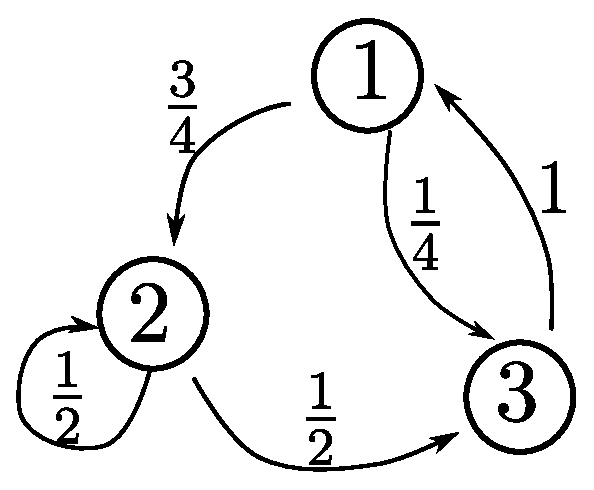
\includegraphics[width=4cm]{H3_2.eps}
\end{figure}

试求
\begin{enumerate}[label=(\arabic*)]
\item 信源的熵率
\item 信源的有效编码及平均码字长。
\end{enumerate}
\begin{solution}\item
\begin{enumerate}[label=(\arabic*)]
\item 该信源的符号集为$\{1,2,3\}$,为平稳1阶马氏链,转移概率矩阵为
$$
\bm{P}=
\begin{bmatrix}
0 & \frac{3}{4} & \frac{1}{4} \\
0 & \frac{1}{2} & \frac{1}{2} \\
1 & 0 & 0
\end{bmatrix}
$$
由此求出平稳分布为
$$
(\pi_1,\pi_2,\pi_3)=(\frac{2}{7},\frac{3}{7},\frac{2}{7})
$$
进一步求出熵率为$H_{\infty}(X)=0.66$
\item 当前状态为1时,对下一状态(只能是2或3)进行0或1的编码;当前状态为2时,对下一状态(只能是2或3)进行0或1的编码;当前状态为3时,下一状态一定是1,状态1的前一状态一定是3,因此状态31可以看成一个整体。这种编码方案平均码长为1。需要区分的是码串开头是1还是3,为此只需用额外1比特约定即可。
\end{enumerate}
\end{solution}
\item 一信源有$ K = x 2^j $($j$ 为整数,$1\leq x \leq 2)$ 个等概率可取的字母。用二元码对此信源字母进行 Huffman 编码,试求此码的平均码长(用$x,j$表示)。
\begin{solution}
当$x=2$时$L(C)=j+1$。当$1\leq x<2$时有$2^j$个码字长度为$j$,$(x-1)2^j$ 个码字长度为$j+1$。平均码长为$j+1-\frac{1}{x}$。
\end{solution}
\item 设有一独立增量过程,在整数时刻时发生数值为+1 或-1 的增量,增量取+1 的概率为0.9,取-1 的概率为 0.1,其初值以等概取自集合$\{-1,0,+1,+2\}$。试求此随机过程的熵率。
\begin{solution}
由离散平稳信源熵率公式和信源的马氏性,得到 
\begin{align*}
H_{\infty} (X)  & = \lim_{n\to \infty} H(X_n |X_{n-1}) \\
H(X_n|X_{n-1})  & = \sum_{a} \Pr(X_{n-1}=a) H(X_n|X_{n-1}=a) \\
& = \sum_{a} \Pr(X_{n-1}=a)(-0.1\log 0.1 - 0.9\log 0.9) \\
& = 0.47
\end{align*}
\end{solution}

\item 设有独立随机序列$\{x_n\},p(x_n = 0) = p,p(x_n = 1)=q,$ 随机序列$\{y_n\}$与$\{x_n\}$的关系为$y_n = x_n \oplus y_{n-1}$,其中$\oplus$为模2和。试求:
\begin{enumerate}[label=(\arabic*)]
\item $\{x_n\}$ 和$\{y_n\}$ 的熵率 $H(X)$ 和 $H(Y)$
\item $H(Y)= 1\mathrm{bit}$/符号的条件
\end{enumerate}
\begin{solution}\item
\begin{enumerate}[label=(\arabic*)]
\item $X$是i.i.d.序列,熵率等于熵,$H(X)=-p\log p-q \log q$。$Y$是两状态的马氏链,转移概率矩阵为$\begin{bmatrix} p & q \\ q & p \end{bmatrix}$。
当$p<1$时,平稳分布为$[\frac{1}{2},\frac{1}{2}]$,此时$H(Y)=H(X)$;当 $p=1$时,$Y_n=Y_{n-1}\Rightarrow H(Y)=0$。
\item 当$p=q=\frac{1}{2}$时。
\end{enumerate}
\end{solution}
\item 设离散无记忆信源的字母表为$\{a_i\},i=1,2,\dots,7$,各字母的出现概率分别为 $0.3,0.25,0.15,0.1,0.1,0.05,0.05$ 试构造二元和三元 Huffmann 码。
\begin{solution}

对于二元 Huffmann 码:
\begin{tikzpicture}[column 3/.style={anchor=west},place/.style={inner sep=1pt}]
\matrix
{
\node {$X$};  &[5mm]\node{码字};&[3mm] \node{概率(按递减排序)};\\
\node {$a_1$};&\node{11};  & \node{0.3}; &[-15mm] \node{0.3};    &[3mm] \node{0.3};       &[3mm] \node{0.3};        &[3mm] \node[place](a10){0.45}; &[3mm] \node[place](b3){0.55}; &[3mm] \node[place](b5){1};\\
\node {$a_2$};&\node{10}; & \node{0.25}; & \node{0.25};         & \node{0.25};           & \node[place]{0.25};     & \node[place](b1){0.3};       &\node[place](b4){0.45};\\
\node {$a_3$};&\node{011}; & \node{0.15}; & \node{0.15};         & \node[place](a5){0.2}; & \node[place](a8){0.25}; & \node[place](b2){0.25};\\
\node {$a_4$};&\node{010}; & \node{0.1}; & \node{0.1};           & \node[place](a7){0.15};       & \node[place](a9){0.2};\\
\node {$a_5$};&\node{001}; & \node{0.1}; & \node[place](a4){0.1};& \node[place](a6){0.1};\\
\node {$a_6$};&\node{0001}; & \node[place](a1){0.05}; & \node[place](a3){0.1};\\
\node {$a_7$};&\node{0000}; & \node[place](a2){0.05}; & \\
};
\draw (a1) -- (a3.west) -- (a2);
\draw (a3.east) -- (a5.west) -- (a4.east);
\draw (a6.east) -- (a8.west) -- (a7.east);
\draw (a8.north east) -- (a10.south west) -- (a9.east);
\draw (b1.east) -- (b3.west) -- (b2.east);
\draw (b4.east) -- (b5.west) -- (b3.east);
\end{tikzpicture}

对于三元 Huffmann 码:
\begin{center}
\begin{tikzpicture}[column 3/.style={anchor=west},place/.style={inner sep=1pt}]
\matrix
{
\node {$X$};  &\node{码字};&[3mm] \node{概率(按递减排序)};\\
\node {$a_1$};&\node{1};  & \node[place]{0.3};             &[-15mm] \node{0.3};    &[5mm] \node[place](a7){0.45};       &[5mm]\node[place](a10){1};\\
\node {$a_2$};&\node{0};  & \node[place]{0.25};            & \node{0.25};          & \node[place](a8){0.3};         \\
\node {$a_3$};&\node{21}; & \node[place]{0.15};            & \node[place](a4){0.2};& \node[place](a9){0.25}; \\
\node {$a_4$};&\node{20}; & \node[place]{0.1};             & \node[place](a5){0.15};     \\
\node {$a_5$};&\node{222}; & \node[place](a3){0.1};         & \node[place](a6){0.1};      \\
\node {$a_6$};&\node{221};& \node[place](a1){0.05}; \\
\node {$a_7$};&\node{220};& \node[place](a2){0.05}; \\
};
\draw (a1.east) -- (a4.west) -- (a2.east);
\draw (a3.east) -- (a4.west);
\draw (a4.east) -- (a7.west) -- (a5.north east);
\draw (a6.east) -- (a7.west);
\draw (a7.east) -- (a10.west) -- (a8.north east);
\draw (a9.east) -- (a10.west);

\end{tikzpicture}
\end{center}
\end{solution}
\end{enumerate}

\end{document}
add `\usepackage{showframe}` just before `\begin{document}` produces the following result on page 3 of `main.pdf`. 

%%% Local Variables:
%%% mode: late\rvx
%%% TeX-master: t
%%% End:
